\section{Experimentation} \label{sec:experimentation}

\subsection{Topology} \label{sec:topology}

The most simple example of a topology involving a client, router, and server
would be a three node setup with links between the client and router and router
and server. However, we would only expect to router cache hits if the same video
was requested multiple times, which while not unlikely due to our
zipf-distribution of video popularity, is a poor representation of reality, and
is also very boring.

We therefore ran our experiments on a more complex topology involving five
clients linked to a single router, which in turn is linked to a server.

\begin{figure}[h]
    \begin{center}
        \begin{tabular}{c}
            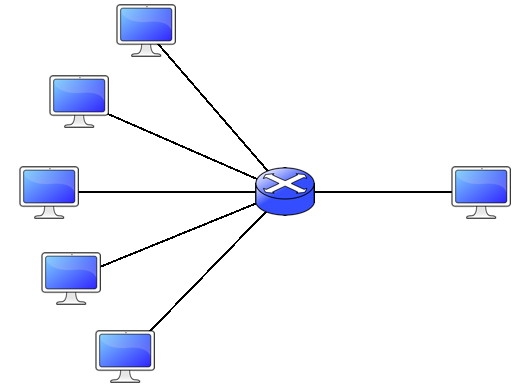
\includegraphics[width=0.45\textwidth]{fig/topology.png} \\
        \end{tabular}
        \caption{Topology for the experiments}
        \label{fig:topology}
    \end{center}
\end{figure}

The bandwidth of the links between the nodes is 10  mbps with
10 ms of latency. With our workload, we do not  see enough traffic for
congestion to affect our results. (RIGHT?????????)



\subsection{Client Application} \label{sec:client}

In order to run our experiments, we had to define a custom client application.
Our client application is simple. First, we pre-generated trace files for each
client, indicating which videos the each client would request, in what order,
and to what ending duration. As we previously mentioned, the videos are chosen
from a zipf distribution of popularity. Because we use these traces, each
experiment we run for different chunk sizes requests the same videos. This
ensures that our results will not have any discrepancies due to random
differences in viewing, but on the downside, our results might not be
representative of the average behavior. We made this compromise in the interest
of time, but ideally, we could have run many randomized experiments multiple
times and found an average.
In order to better replicate real-world video streaming applications, we define
a buffer which is 0.3 times the length of the video. Instead of beginning the
simulating watching of the video once the first chunk is received, which we had
done originally, we begin the watching of the video once the buffer is full for
the first time. Once the video has begun to be watched, we track the current
play time of the video and the amount of data fetched separately. The buffer
slides along with the current play time such that the client tries to always
have the next 30\% of the chunks of the video pre loaded. The client would be
considered to be in a buffering state if the current play time catches up to the
last chunk fetched in the buffer.

Once a client reads in a video to watch from its corresponding trace file, it
begins requesting chunks of the video to the server by sending interests. The
clients do not specify the size of the chunk in the requests; this is defined in
the server application. Instead, the client determines the size of the chunk by
checking the size of the data received. Once data is received, the client
updates the buffer, checks if its buffer is full, and requests another chunk if
it is not. If it is full, the client waits until another chunk’s worth of play
time has passed, and then requests another chunk.

\subsection{Server Application} \label{sec:server}

The server waits for an interest to be received, and when it does, it returns of
chunk to the client, which is a data buffer of the chunk size being measured for
that experiment. The content of the chunk is currently not checked by either the
server or the client, so there is no content verification in place. This is
really the extent of what the server does.

\subsection{Router} \label{sec:router}

The router is not something we programmed, but we did configure it. As was
mentioned before, the size of the router is defined in terms of the number of
packets, rather than an absolute size. Therefore, we set the size to be equal to
7 MB, a value small enough that on average, an entire video could not exist in
the cache at one time.

We also used the router to observe the pending interests table, a data structure
which tracks which interests were received but not yet served by the router.
This is unique to these content centric network models.

\subsection{MTU} \label{sec:mtu}

ndnSIM has a default MTU value of 1500 bytes, which is in line with the maximum
packet size allowed by ethernet. Unfortunately, this means that if we experiment
with chunks larger than this value, ndnSIM automatically breaks them up into
multiple packets, which are then individually cached by the content store. If we
then want to evict a logical chunk from the cache, we have to modify ndnSIM to
ensure that all of the chunks corresponding to the chunk is evicted. 

In order to circumvent this complication, we configured ndnSIM to have an MTU
much larger than any of the chunk sizes we experimented with. Although this does
not model the real world perfectly, we felt this was an acceptable compromise
because it would allow us to trust the cache to behave as we expected.

\subsection{Batching} \label{sec:batching}

In some initial runs of our experiment, we did not implement any batching of
requests by the client. Individual chunks were requested in order, one after the
other. Unsurprisingly, certain metrics we chose like start-up time suffered
miserably as RTT for the packets (40 ms, with our particular topology) consumed
the vast majority of the time before the initial buffer filled and the video
started being watched.

For later experiments, we implemented batching on the client. Instead of
individual interests, the client computes which chunks in the buffer are not yet
fetched, and sends individual interests for those chunks all at once. Once it
receives all of the data for this batch of requests, it repeats the process. The
effects of this are quantified in the results section.
